\documentclass[12pt, letterpaper]{article}
\usepackage[utf8]{inputenc}
\usepackage{indentfirst}
\usepackage{amsfonts} 
\usepackage{amsmath}
\usepackage{amssymb}
\usepackage{graphicx}
\usepackage{hyperref}

\hypersetup{
    colorlinks=true,
    linkcolor=,
    filecolor=magenta,      
    urlcolor=cyan,
    pdftitle={Teste 5 - MC758},
    pdfpagemode=FullScreen,
    pdfsubject={},
    pdfauthor={Rian Radeck Santos Costa},
    pdfkeywords={}
    }
\graphicspath{ {images/} }


\title{Teste 5 - MC758}
\author{Rian Radeck Santos Costa - 187793}
\date{02 de Outubro de 2022}

\begin{document}

\maketitle
\footnotetext{\textit{Todos os exercícios se referem ao livro ``Algorithmic Game Theory''.}}
\newpage

\section{Exercício 20.2}
	Dado $m \in \mathbb{N}$ vamos escolher os pesos das nossas tarefas da seguinte maneira:

	\begin{center}
	\begin{tabular}{||c c c c c c||} 
		\hline
		$l(1)$ & $l(2)$ & $l(3)$ & $\cdots$ & $l(m - 1)$ & $l(m)$ \\ 
		\hline\hline
		$m$ & $m - 1$ & $m - 2$ & $\cdots$ & 2 & 1 \\
		\hline
		1 & 2 & 3 & $\cdots$ & $m - 1$ & $m$ \\ 
		\hline
	\end{tabular}
	\end{center}

	Aqui $l(j)$ representa a carga da máquina $j$, sendo assim a atribuição mostrada é uma de custo ótimo opt$(J) = m + 1$.

	Agora precisamos encontrar uma atribuição de custo $2m$ que seja um equilíbrio, para isso vamos ``shiftar'' a primeira linha das tarefas uma vez para esquerda

	\begin{center}
	\begin{tabular}{||c c c c c c||} 
		\hline
		$l(1)$ & $l(2)$ & $l(3)$ & $\cdots$ & $l(m - 1)$ & $l(m)$ \\ 
		\hline\hline
		$m - 1$ & $m - 2$ & $m - 3$ & $\cdots$ & 1 & m \\
		\hline
		1 & 2 & 3 & $\cdots$ & $m - 1$ & $m$ \\ 
		\hline
	\end{tabular}
	\end{center}

	Veja que todas as máquinas agora possuem carga $m$ exceto a última que possui $2m$ e isso é um equilíbrio. Assim o custo dessa atribuição é cost$(A) = 2m$.

	Então podemos concluir que para qualquer $m \in \mathbb{N}$ existe $A$ tal que $$\textrm{cost}(A) = \left(2 - \frac{2}{m + 1} \right) \textrm{opt}(J)$$onde $J$ é um jogo de balanceamento de cargas de máquinas idênticas com $m$ máquinas e $2m$ tarefas e $A$ é uma atribução desse jogo.

\section{Exercício 20.4}
	Considere a máquina 1 com velocidade 1 e a máquina 2 com velocidade $s$. Uma observação muito importante a ser feita é que o jogo é simétrico, então em qualquer equilíbrio o perfil de estratégia dos jogadores será igual e consequentemente sua utilidade será a mesma.
	\subsection{Letra (a)}
		Vamos analisar os casos separadamente, então se $s \leq \frac{1}{2}$ nenhuma tarefa será alocada para a máquina 2, já que a carga dessa máquina seria pelo menos $l(2) \geq 1/(1 / 2) = 2$ (quando uma das tarefas estiver lá), porém a carga da máquina 1 é no máximo 2 (quando ambas as tarefas estão lá), logo não faz sentido uma tarefa estar na máquina 2. Assim podemos concluir que o equilíbrio misto de Nesh seria na verdade um equilíbrio puro de Nesh se $s \leq \frac{1}{2}$.

		Vamos ao segundo caso, $s \geq 2$. Nesse caso nenhuma tarefa seria alocada para a máquina 1 já que a máquina 2 consegue terminar seu trabalho antes ou no mesmo tempo da máquina 1, mesmo se todas as tarefas estiverem lá. Sendo assim, concluimos também que o equilíbrio para esse caso é puro.
	\subsection{Letra (b)}
		Utilizando o fato de que o perfil de estratégias dos jogadores serão iguais vamos considerar que a probabilidade de eles escolherem a máquina 1 é $p$, portanto o perfil de estratégia de ambos os jogadores será $(p, 1 - p)$. Vamos então calcular o custo de um jogador se ele escolher cada uma das máquinas:
		\begin{itemize}
			\item{Máquina 1: $p + 1$}
			\item{Máquina 2: $\frac{(1 - p) + 1}{s} = \frac{2 - p}{s}$}
		\end{itemize}

		Como queremos encontrar um equilíbrio misto, sabemos que a probabilidade de escolha entre a máquina 1 e a 2 tem que ser a mesma, sendo assim o custo das máquinas tem que ser o mesmo portanto
		$$
			p + 1 = \frac{2 - p}{s} \Leftrightarrow p = \frac{2 - s}{1 + s}
		$$

		Então nosso perfil de estratégias para ambos os jogadores será
		$$
			(p, 1 - p) = \left(\frac{2 - s}{1 + s}, \frac{2s - 1}{1 + s} \right)
		$$

\section{Exercício 19.4}
	Dado um jogo de conexão local, tome dois vértices $u$ e $v$ tal que a distâcia entre eles é pelo menos $2k$ para algum $k \geq 1$.
	Se algum deles, digamos $u$, paga pela aresta ${u, v}$, sabemos que seu custo aumenta de $\alpha$, porém todos os vértice no antigo caminho de $u$ a $v$ que estavam mais próximos de $v$, vão ter sua distância a $u$ reduzida de algum fator (parte verde da imagem \ref{img:path}) e algo similar acontecerá a $v$.
	\begin{figure}[h]
		\label{img:path}
        \centering
        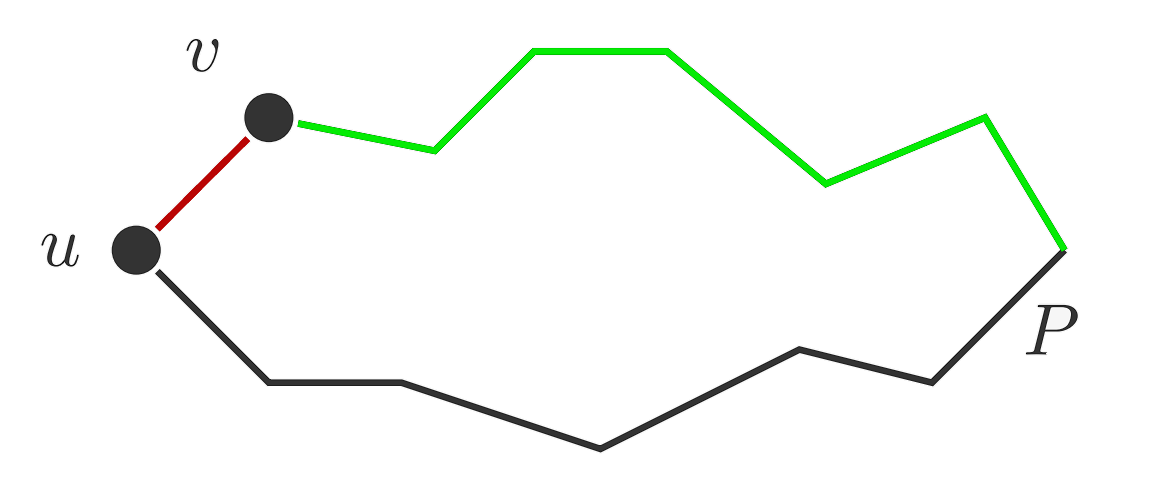
\includegraphics[width=0.6\textwidth]{path.png}
        \\{Aresta vermelha diminui a distância de $u$ e $v$ para alguns vértices}
    \end{figure}

    O fator de economia do custo de $u$ será pelo menos
    $$
    \sum_{n = 1}^{k}{2n - 1} = k^2
    $$ 
    já que $k$ é o mínimo número de vértices que terão suas distâncias afetadas até $u$.

    Podemos concluir então que se existe caminho maior ou igual a $2k$ em um jogo de conexão global, esse jogo não é um equilíbrio, já que $d(u, v) \geq 2k > 2\sqrt{\alpha}$.

\section{Exercício 19.7}
	Considere um equilíbrio, o diâmetro $d$ do grafo tem tamanho máximo $n$ vértices. Dessa forma, se o grafo não for uma árvore, quando retirarmos uma aresta dele que não seja uma ponte, economizaremos o preço daquela aresta ($\alpha > n^2$) e o custo de no máximo $n$ vértices será aumentado de no máximo $d$, portanto o custo aumentará de no máximo $nd \leq n^2$. Isso significa que tal aresta não existia (custo do grafo diminuiu após a remoção de tal aresta), já que estávamos em um equilíbrio, portanto nossa suposição inicial estava errada e todo equilíbrio com $\alpha > n^2$ é uma árvore.

	Agora veja que o pior caso é quando temos um grafo linear (cada vértice tem um pai diferente), dessa maneira cada um dos $n^2$ caminhos têm a quantidade máxima de vértices entre eles. A soma exata dos caminhos será na verdade
	$$
	\sum_{k = 3}^{n}{(k - 1)(k - 2)} = n^3 / 3 - n^2 + 2n / 3 \leq n^3
	$$

	Já no custo ótimo nosso grafo será uma estrela e a soma dos caminhos é $2(n-1)(n-2) + 2(n - 1) \leq n^2$. Portanto o preço da anarquia será sempre limitada pelo fator $n^3 / n^2 = n$.

\section{Exercício 19.9}
	Suponha que em um jogo de conexão global $J$, PoA($J$) $> n \therefore \exists$ $S$ tal que $ \textrm{cost}(S) > n \textrm{ cost}(S')$, onde $S'$ é o perfil de estratégias da estratégia ótima.

	Como o custo de uma uma estratégia $S = (P_1, P_2, \ldots, P_n)$ é a soma dos custos dos seus jogadores, deve existir algum jogador $i \in [n]$ tal que cost$_i(S) > \textrm{cost}_i(S')$. Contudo, o caminho $P_i'$ da estratégia ótima satisfaz cost$_i(S*) \leq \textrm{cost}(S')$, para toda estratégia $S*$. Isso se deve ao fato de que o custo da função social também é o somatório dos custos máximos para cada aresta, e que o caminho $P_i'$ é um subconjunto das arestas de $S'$. Então se um jogador muda a sua estratégia para $P_i'$, ele diminui seu custo em até cost$(S')$. O que implica que S não é um equilíbrio de Nesh.

\section{Exercício 19.11 (a)}
	\begin{itemize}
		\item{$G = (V, E)$: um digrafo.}
		\item{$(s_i, t_i)$: pares de vértices dos jogadores $i = 1, 2, \ldots, k$.}
		\item{$S = (P_1, P_2, \ldots, P_k)$ um perfil de estratégias.}
		\item{$k_e$ o número de caminhos em $S$ que usam $e$.}
	\end{itemize}

	Como a função de custo do caminho do jogador $i$ é definida por
	$$
		\textrm{cost}(P_i) = \sum_{e \in P_i}{l_e(k_e)}
	$$
	onde $l_e$ é uma função de latência para a aresta $e$, podemos achar sua função potencial
	$$
		\psi_e(S) = \sum_{k = 1}^{k_e}{l_e(k)}
	$$$$
		\psi(S) = \sum_{e \in E}{\psi_e(S)}
	$$

	Agora precisamos provar que existe $P_i' \neq P_i$ um caminho alternativo para $i$ que nos dá $S' = (S_{-i}, P_i')$ o perfil de estratégias com o novo caminho de $i$, tal que
	$$
		\psi(S) - \psi(S') = \textrm{cost}_i(S) - \textrm{cost}_i(S')
	$$

	Vamos analisar os três possíveis casos para uma aresta $e \in E$.
	\begin{itemize}
		\item{Se $e$ está em $P_i$ mas não em $P_i'$, então}
		\begin{itemize}
			\item{$\psi_e(S') = \psi_e(S) - l_e(k_e)$}
			\item{e $i$ deixou de pagar $l_e(k_e)$.}
		\end{itemize}
		\item{Se $e$ está em $P_i'$ mas não em $P_i$, então}
		\begin{itemize}
			\item{$\psi_e(S') = \psi_e(S) + l_e(k_e + 1)$}
			\item{e $i$ passa de pagar $l_e(k_e + 1)$ a mais.}
		\end{itemize}
		\item{Caso contrário, $\psi_e(S) = \psi_e(S')$.}
	\end{itemize}

	Assim sendo $\psi(S) - \psi(S') = \textrm{cost}_i(S) - \textrm{cost}_i(S')$.

\end{document}